\documentclass{beamer}
\usepackage{relsize}
\usepackage{color}

\usepackage{listings}
\usetheme{CambridgeUS}
%\usepackage{beamerthemesplit} % new 
\usepackage{enumitem}
\usepackage{amsmath}                    % See geometry.pdf to learn the layout options. 
\usepackage{amsthm}                   % See geometry.pdf to learn the layout options. There 
\usepackage{amssymb}                    % See geometry.pdf to learn the layout options. 
\usepackage[utf8]{inputenc} 
\usepackage{graphicx}
\usepackage[english,bulgarian]{babel}

\lstset{language=C++,
                basicstyle=\ttfamily,
                keywordstyle=\color{blue}\ttfamily,
                stringstyle=\color{red}\ttfamily,
                commentstyle=\color{green}\ttfamily,
                morecomment=[l][\color{magenta}]{\#}
}

\newtheorem{mydef}{Дефиниция}[section]
\newtheorem{lem}{Лема}[section]
\newtheorem{thm}{Твърдение}[section]

\DeclareMathOperator{\restrict}{\upharpoonright}

\setitemize{label=\usebeamerfont*{itemize item}%
  \usebeamercolor[fg]{itemize item}
  \usebeamertemplate{itemize item}}

\setbeamercovered{transparent}



\begin{document}
\title[Обектно ориентирано програмиране]{Конструктор за копиране} 
\author{Калин Георгиев} 
\frame{\titlepage} 

\section{Споделяне на памет} 


\begin{frame}
\centerline{Проблемът със споделянето на памет}
\end{frame}


\begin{frame}[fragile]
\frametitle{Обект и динамична памет}
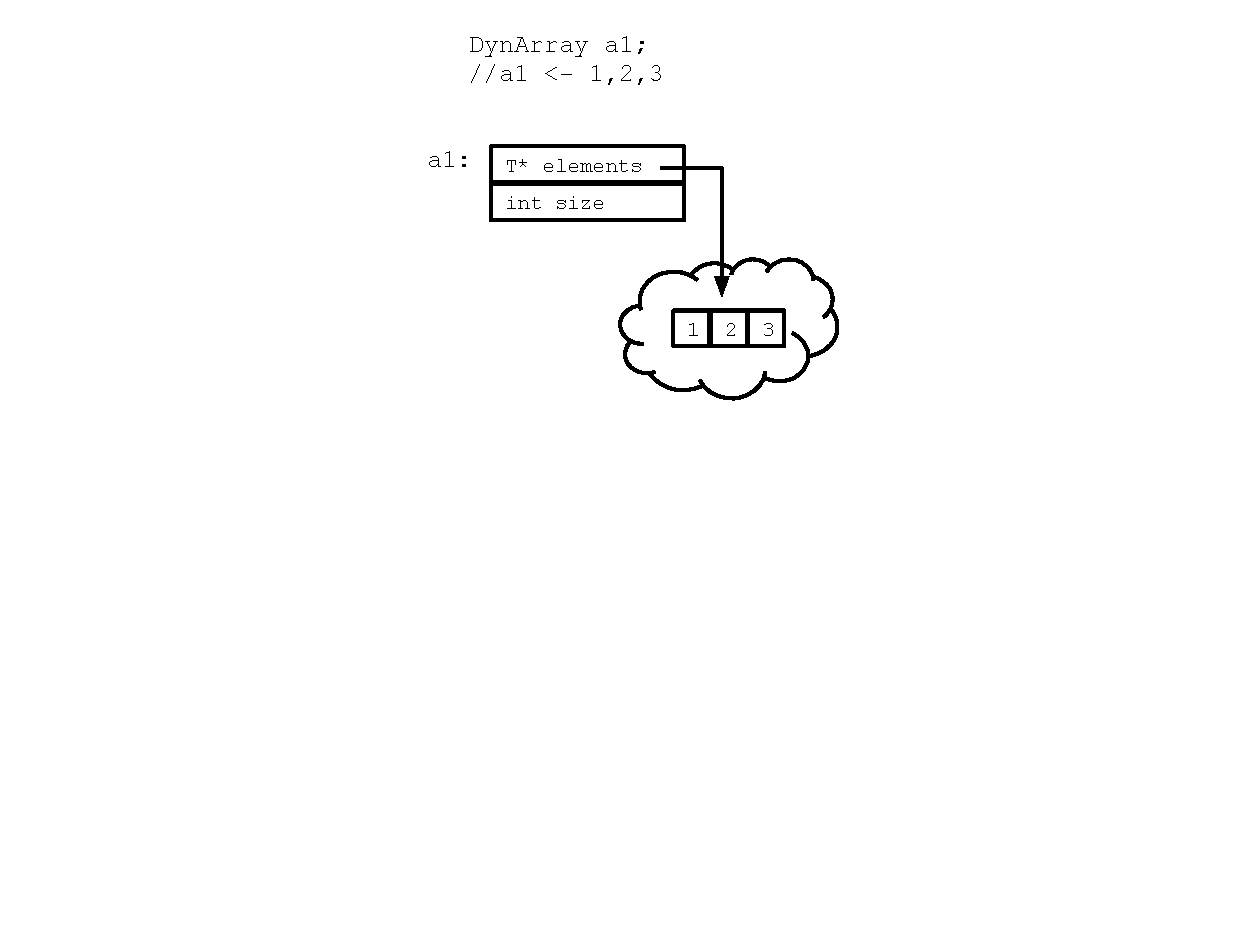
\includegraphics[width=12.5cm]{images/memshare_01}
\end{frame}

\begin{frame}[fragile]
\frametitle{Инициализация чрез копиране}
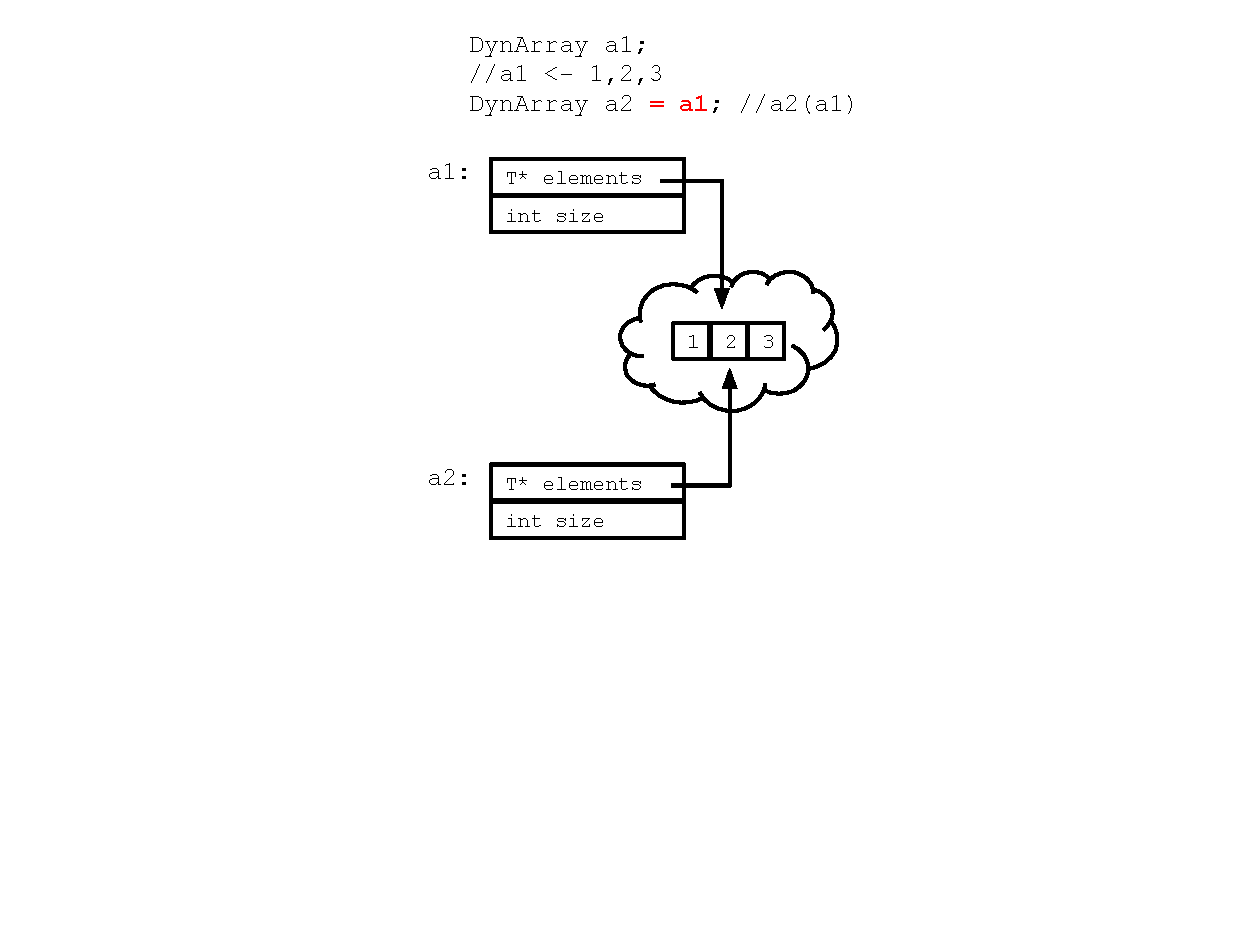
\includegraphics[width=12.5cm]{images/memshare_02}
\end{frame}

\begin{frame}[fragile]
\frametitle{Операциите се отразяват на ``общата памет''}
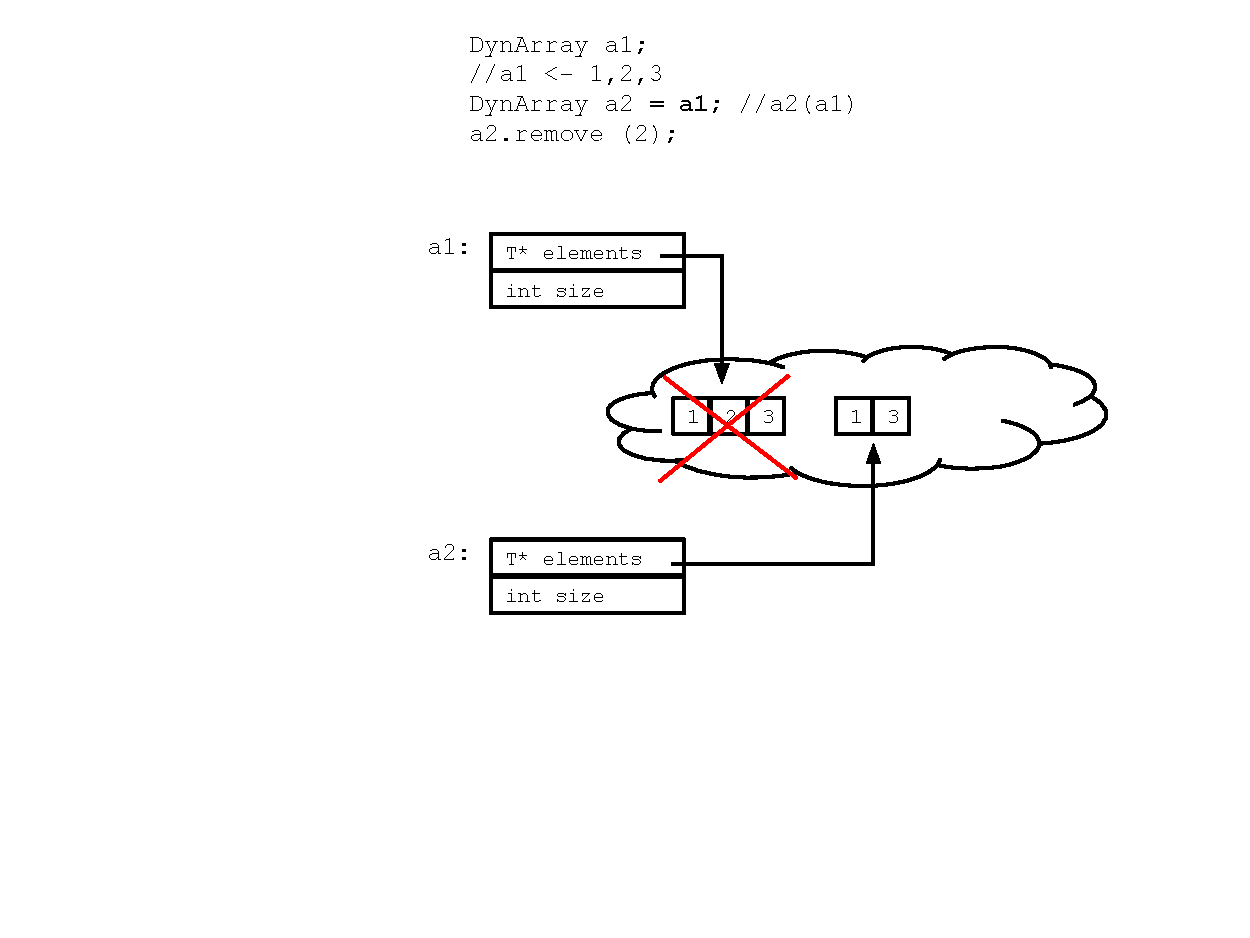
\includegraphics[width=12.5cm]{images/memshare_03}
\end{frame}

\begin{frame}[fragile]
\frametitle{Операциите се отразяват на ``общата памет''}
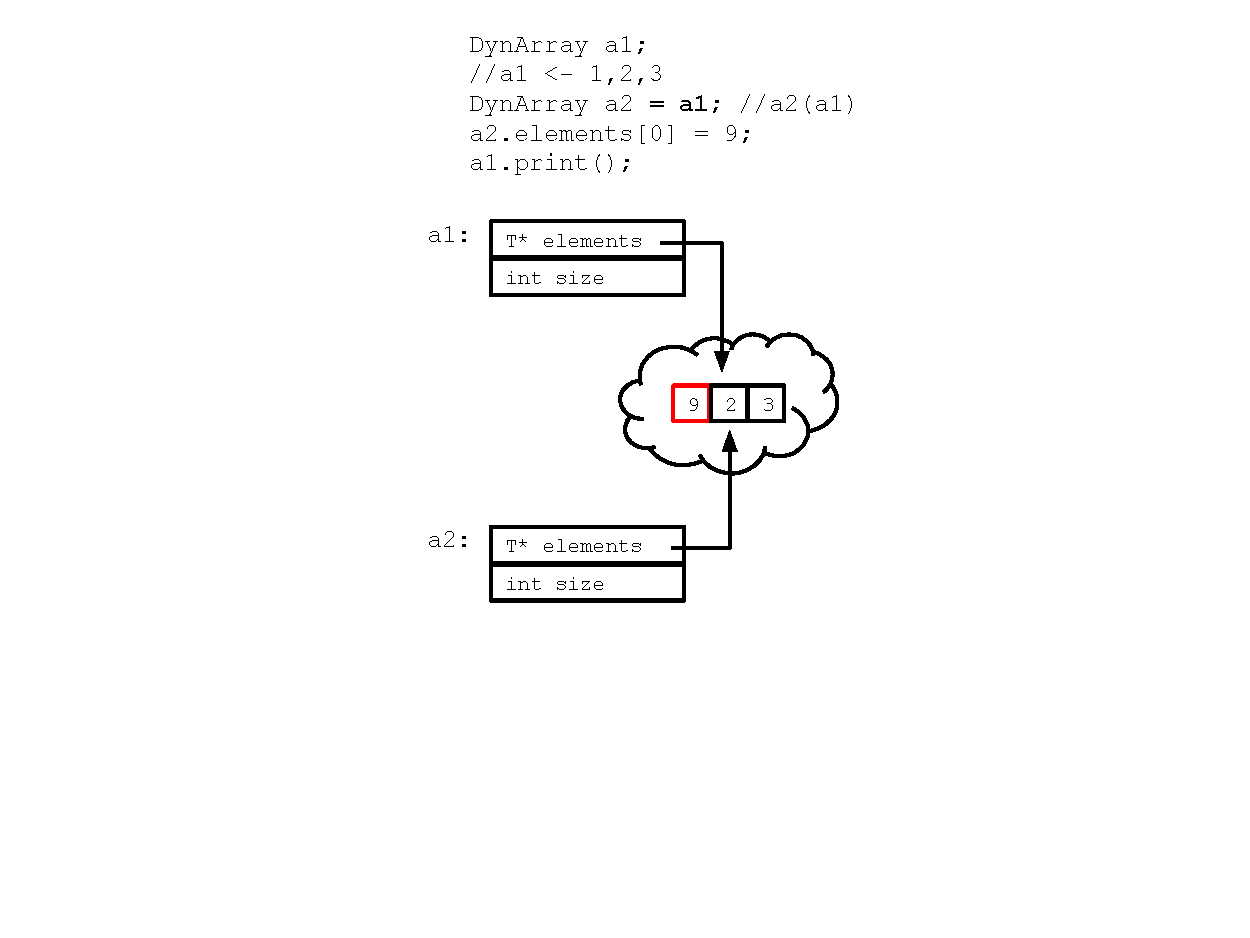
\includegraphics[width=12.5cm]{images/memshare_04}
\end{frame}

\begin{frame}[fragile]
\frametitle{Решението е ``истинско'' копиране}
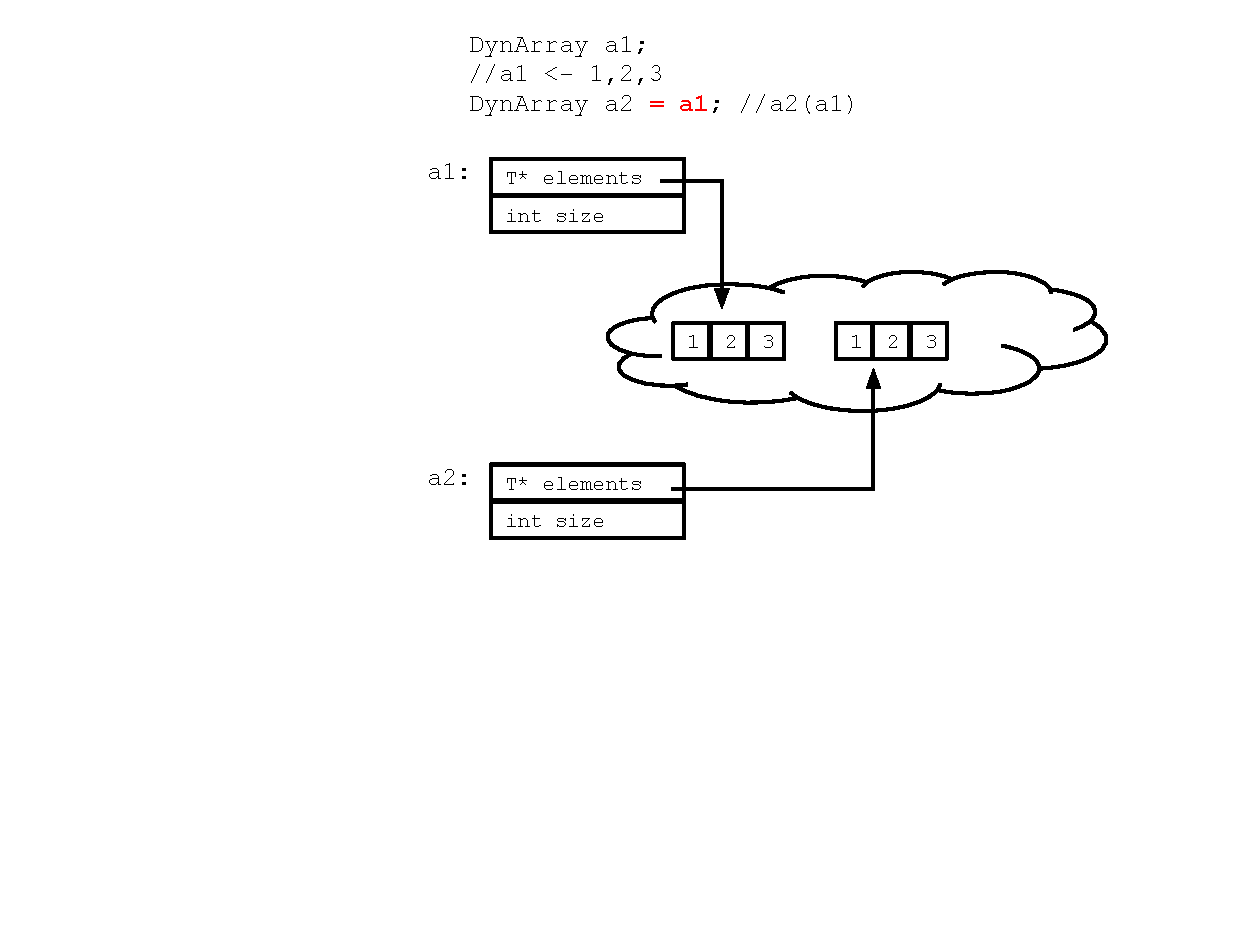
\includegraphics[width=12.5cm]{images/memshare_05}
\end{frame}



\section{Копиране} 


\begin{frame}
\centerline{Случаи на копиране}
\end{frame}

\begin{frame}[fragile]
\frametitle{Пример}


\begin{flushleft}
\relscale{0.75}
\begin{lstlisting}
class Point
{
  public:
  double x,y;

  Point (){x=0;y=0;}
  Point (double _x, double _y){x=_x; y=_y;}
  Point (Point &p) {x=p.x; y=p.y;}
  Point (double _x) {x=y=_x};

};
\end{lstlisting}  
\end{flushleft}

\end{frame}


\begin{frame}[fragile]
\frametitle{Опростена схема}
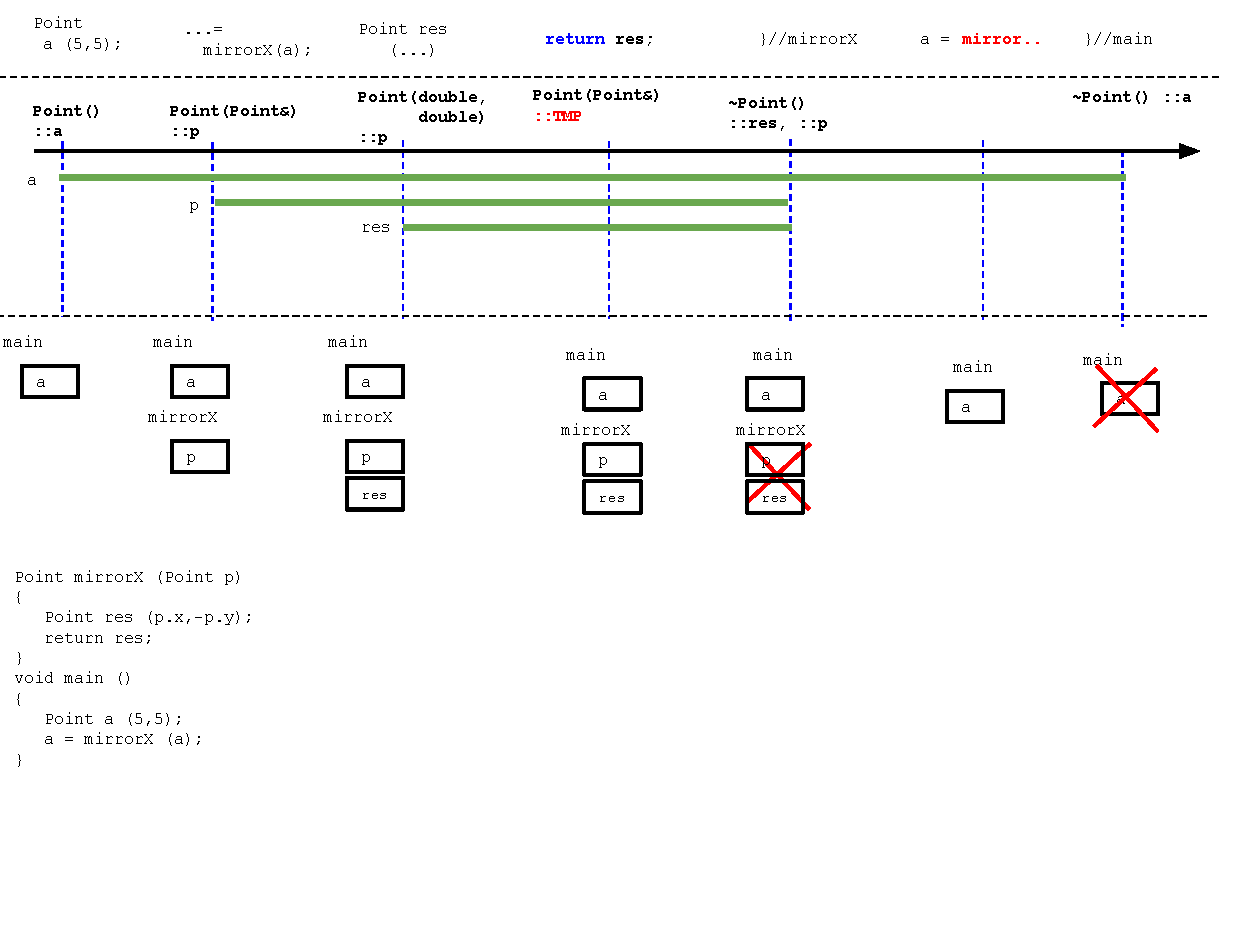
\includegraphics[width=12.5cm]{images/lc_return_simple}
\end{frame}

\begin{frame}[fragile]
\frametitle{Пълна схема}
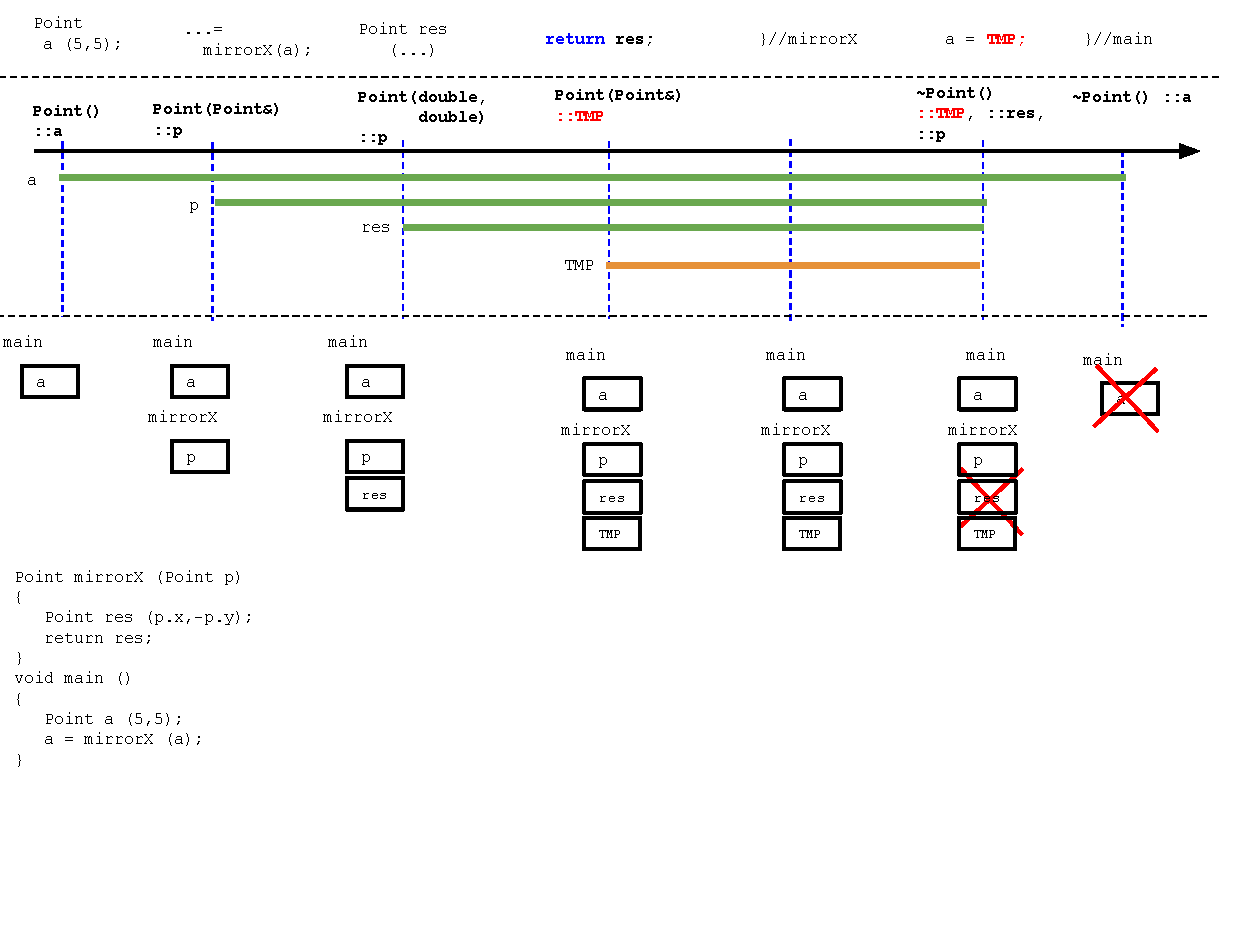
\includegraphics[width=12.5cm]{images/lc_return_full}
\end{frame}

\begin{frame}[fragile]
\frametitle{Сравнение}
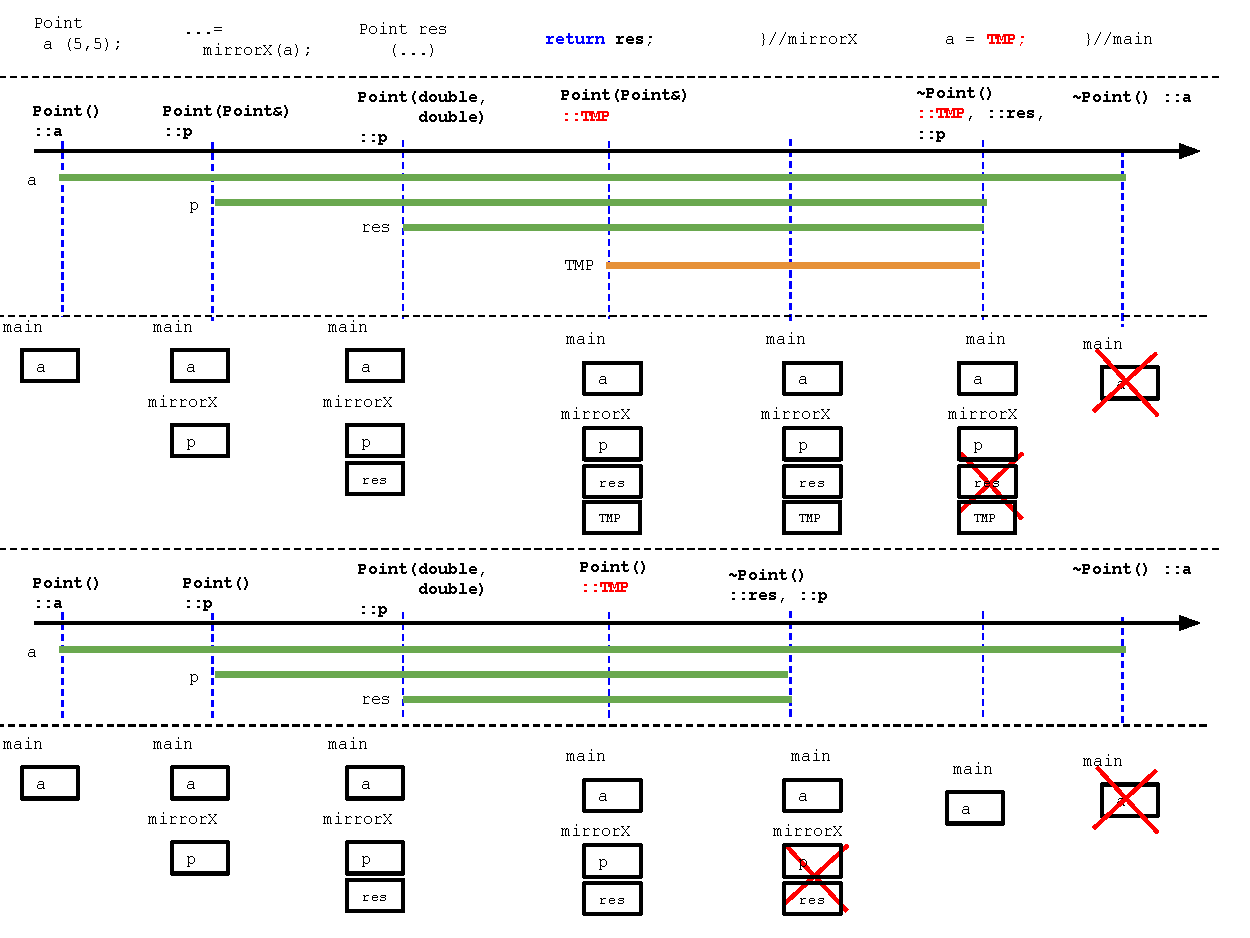
\includegraphics[width=9.5cm]{images/lc_return_dual}
\end{frame}


\begin{frame}
\centerline{Благодаря за вниманието!}
\end{frame}


\end{document}



\begin{columns}[t]
  \begin{column}{0.55\textwidth}

  \end{column}
  \begin{column}{0.45\textwidth}

  \end{column}
\end{columns}
